%%%%%%%%%%%%%%%%%%%%%%%%%%%%%%%%%%%%%%%%%%%%%%%%%%%%%%%%%%%%%%%%%%%%
%% I, the copyright holder of this work, release this work into the
%% public domain. This applies worldwide. In some countries this may
%% not be legally possible; if so: I grant anyone the right to use
%% this work for any purpose, without any conditions, unless such
%% conditions are required by law.
%%%%%%%%%%%%%%%%%%%%%%%%%%%%%%%%%%%%%%%%%%%%%%%%%%%%%%%%%%%%%%%%%%%%
\PassOptionsToPackage{svgnames}{xcolor}

\documentclass[
  digital, %% This option enables the default options for the
           %% digital version of a document. Replace with `printed`
           %% to enable the default options for the printed version
           %% of a document. 'digital'/'printed'
  oneside, %% This option enables double-sided typesetting. Use at
           %% least 120 g/m² paper to prevent show-through. Replace
           %% with `oneside` to use one-sided typesetting; use only
           %% if you don’t have access to a double-sided printer,
           %% or if one-sided typesetting is a formal requirement
           %% at your faculty.
  table,   %% This option causes the coloring of tables. Replace
           %% with `notable` to restore plain LaTeX tables.
  nolof,     %% This option prints the List of Figures. Replace with
           %% `nolof` to hide the List of Figures.
  nolot,     %% This option prints the List of Tables. Replace with
           %% `nolot` to hide the List of Tables.
  %% More options are listed in the user guide at
  %% <http://mirrors.ctan.org/macros/latex/contrib/fithesis/guide/mu/fi.pdf>.
]{fithesis3}
%% The following section sets up the locales used in the thesis.
\usepackage[resetfonts]{cmap} %% We need to load the T2A font encoding
\usepackage[T1,T2A]{fontenc}  %% to use the Cyrillic fonts with Russian texts.
\usepackage[
  main=english, %% By using `czech` or `slovak` as the main locale
                %% instead of `english`, you can typeset the thesis
                %% in either Czech or Slovak, respectively.
  english, german, russian, czech, slovak %% The additional keys allow
]{babel}        %% foreign texts to be typeset as follows:
%%
%%   \begin{otherlanguage}{german}  ... \end{otherlanguage}
%%   \begin{otherlanguage}{russian} ... \end{otherlanguage}
%%   \begin{otherlanguage}{czech}   ... \end{otherlanguage}
%%   \begin{otherlanguage}{slovak}  ... \end{otherlanguage}
%%
%% For non-Latin scripts, it may be necessary to load additional
%% fonts:
\usepackage{paratype}
\def\textrussian#1{{\usefont{T2A}{PTSerif-TLF}{m}{rm}#1}}
%%
%% The following section sets up the metadata of the thesis.
\thesissetup{
    date          = \the\year/\the\month/\the\day,
    university    = mu,
    faculty       = fi,
    type          = mgr,
    author        = Bc. Andrej Staruch,
    gender        = m,
    advisor       = {RNDr. Marek Kumpošt, Ph.D.},
    title         = {Aplikace pro detekci phishing útoků na základě testování URL},
    TeXtitle      = {Aplikace pro detekci phishing útoků na základě testování URL},
    keywords      = {phishing detection, Phishtank, security, cpp, 
javascript, URL tests, Trusted Network Solutions},
    TeXkeywords   = {phishing detection, Phishtank, security, cpp, 
javascript, URL tests, Trusted Network Solutions},
    abstract      = {The goal of this master's thesis is to design and implement a system, which will compute potential risk for a given URL. The computation of potential risk is based on extendable series of individual test suites, and the result of weighted tests is a number called 'phishing score'. Based on this number, the application can automatically allow or block the given communication. Optionally, the end user could be warned and decide if he wants to proceed to this website.
    },
    % thanks        = {These are the acknowledgements for my thesis, Mgr. Karol Kubanda, učo 143339 (konzultant) },
    bib           = example.bib,
}
% http://blog.chapagain.com.np/latex-numbering-subsubsection-and-showing-it-in-table-of-contents/


\usepackage{makeidx}      %% The `makeidx` package contains
\makeindex                %% helper commands for index typesetting.
%% These additional packages are used within the document:
\usepackage{paralist} %% Compact list environments
\usepackage{amsmath}  %% Mathematics
\usepackage{amsthm}
\usepackage{amsfonts}
\usepackage{url}      %% Hyperlinks
\PassOptionsToPackage{hyphens}{url}\usepackage{hyperref}
\usepackage[footnotes,definitionLists,hashEnumerators,smartEllipses,hybrid]{markdown}
\usepackage{listings} %% Source code highlighting
\usepackage{booktabs}
\usepackage{tabularx}
\usepackage{dirtree}
\usepackage{csquotes}
\usepackage{pgfplots} % barplot graph
\usepgfplotslibrary{dateplot}
\pgfplotsset{compat=1.12}

% https://tex.stackexchange.com/questions/112631/how-to-write-multiple-line-caption-with-figure
\usepackage{caption}

% https://tex.stackexchange.com/questions/9796/how-to-add-todo-notes
\usepackage[colorinlistoftodos,textsize=tiny]{todonotes}
\usepackage{xargs}                      % Use more than one optional parameter in a new commands

\newcommandx{\unsure}[2][1=]{\todo[linecolor=red,backgroundcolor=red!25,bordercolor=red,#1]{#2}}
\newcommandx{\change}[2][1=]{\todo[linecolor=blue,backgroundcolor=blue!25,bordercolor=blue,#1]{#2}}
\newcommandx{\info}[2][1=]{\todo[linecolor=OliveGreen,backgroundcolor=OliveGreen!25,bordercolor=OliveGreen,#1]{#2}}
\newcommandx{\improvement}[2][1=]{\todo[linecolor=Plum,backgroundcolor=Plum!25,bordercolor=Plum,#1]{#2}}
\newcommandx{\thiswillnotshow}[2][1=]{\todo[disable,#1]{#2}}
%

% https://tex.stackexchange.com/questions/120336/adding-several-labels-year-month-to-a-graph-in-pgfplots
\makeatletter
\long\def\ifnodedefined#1#2#3{%
    \@ifundefined{pgf@sh@ns@#1}{#3}{#2}%
}
\makeatother

%% https://tex.stackexchange.com/questions/2504/beamer-blocks-in-ordinary-article-style-document
\usepackage{tcolorbox}
\usepackage{lipsum}
\tcbuselibrary{skins,breakable}
\usetikzlibrary{shadings,shadows}

% Numbering also for subsubsection
% fithesis/style/mu/fithesis-base.sty:498:\setcounter{secnumdepth}{3}
% \setcounter{secnumdepth}{3} <- this is overrided in fithesis-base


\newenvironment{myexampleblock}[1]{%
    \tcolorbox[beamer,%
    noparskip,breakable,
    colback=LightGreen,colframe=DarkGreen,%
    colbacklower=LimeGreen!75!LightGreen,%
    title=#1]}%
    {\endtcolorbox}

\newenvironment{myalertblock}[1]{%
    \tcolorbox[beamer,%
    noparskip,breakable,
    colback=LightCoral,colframe=DarkRed,%
    colbacklower=Tomato!75!LightCoral,%
    title=#1]}%
    {\endtcolorbox}

\newenvironment{myblock}[1]{%
    \tcolorbox[beamer,%
    noparskip,breakable,
    colback=LightBlue,colframe=DarkBlue,%
    colbacklower=DarkBlue!75!LightBlue,%
    title=#1]}%
    {\endtcolorbox}
    
\newcounter{feature}
\newenvironment{feature}[1]{\stepcounter{feature}%
    \tcolorbox[beamer,%
    noparskip,breakable,
    colback=LightBlue,colframe=DarkBlue,%
    colbacklower=DarkBlue!75!LightBlue,%
    title=Feature~\thefeature: #1]}%
    {\endtcolorbox}
    



\lstset{
  basicstyle      = \ttfamily,%
  identifierstyle = \color{black},%
  keywordstyle    = \color{blue},%
  keywordstyle    = {[2]\color{cyan}},%
  keywordstyle    = {[3]\color{olive}},%
  stringstyle     = \color{teal},%
  commentstyle    = \itshape\color{magenta}}
\usepackage{floatrow} %% Putting captions above tables
\floatsetup[table]{capposition=top}

%%% author on next line
%%% https://tex.stackexchange.com/questions/351733/csquotes-and-beamer-citation-for-blockquote-flush-right-on-separate-line?noredirect=1
\renewcommand{\mkblockquote}[4]{#1#2\newline\null\hfill\rule{0.5\textwidth}{0.1pt}\newline\null\hfill\footnotesize{#4#3}}


\usepackage{listings}
\usepackage{xcolor}  % Coloured text etc.
 
\definecolor{codegreen}{rgb}{0,0.6,0}
\definecolor{codegray}{rgb}{0.5,0.5,0.5}
\definecolor{codepurple}{rgb}{0.58,0,0.82}
\definecolor{backcolour}{rgb}{0.95,0.95,0.92}
 
\lstdefinestyle{mystyle}{
    backgroundcolor=\color{backcolour},   
    commentstyle=\color{codegreen},
    keywordstyle=\color{magenta},
    numberstyle=\tiny\color{codegray},
    stringstyle=\color{codepurple},
    basicstyle=\ttfamily\footnotesize,
    breakatwhitespace=false,         
    breaklines=true,                 
    captionpos=b,                    
    keepspaces=true,                 
    numbers=left,                    
    numbersep=5pt,                  
    showspaces=false,                
    showstringspaces=false,
    showtabs=false,                  
    tabsize=2
}
 
\lstset{style=mystyle}
 
    
\begin{document}



\chapter{Introduction}

\setlength {\marginparwidth }{2cm}

\nocite{apwg-2012-4}
\nocite{apwg-2013-1}
\nocite{apwg-2013-2}
\nocite{apwg-2013-3}
\nocite{apwg-2013-4}
\nocite{apwg-2014-1}
\nocite{apwg-2014-2}
\nocite{apwg-2014-3}
\nocite{apwg-2014-4}
\nocite{apwg-2015-1}
\nocite{apwg-2015-4}
\nocite{apwg-2016-1}
\nocite{apwg-2016-2}
\nocite{apwg-2016-3}
\nocite{apwg-2016-4}
\nocite{apwg-2017-1}
\nocite{apwg-2017-3}
\nocite{apwg-2017-4}
\nocite{apwg-2018-1}
\nocite{apwg-2018-2}
\nocite{apwg-2018-3}
\nocite{apwg-2018-4}
\nocite{apwg-2019-1}
\nocite{apwg-2019-2}

In today's world, the threat of a cyber attack can't be ignored. There are a plethora of companies that try to protect their customers from potential damage, such as getting infected by a virus, getting ransomware or malware or protect their business intelligence.

This thesis is concerned with another part of the cyber crime called phishing. Phishing is a social engineering attack to obtain sensitive information such as user names, passwords, credit card details, bank account credentials for malicious reasons.  Because of a large attack vector, there isn't a reliable way or a tool to prevent such an attack consistently in every sector.

This thesis will review several ways to detect a phishing attack, implement some of them and test them in the production environment with an association with a Trusted Network Solutions company. The final software could be easily used with another proxy or tool.

First of all, we'll look around current market for existing solutions for phishing protection and compare them. After that, we will look for academic papers with phishing oriented thematic and review different approaches and choose suitable ones. Following these steps, we will design and implement phishing detection system. After that, we will test it on real customer traffic and conclude to result whether security of users has increased or not.

Designing an anti-phishing system has similar character as designing an anti-virus system - we are trying to protect user before malicious attempts of an attacker but as we can see, users are still infected when they are using anti-virus, so designing correct and powerful anti-phishing system is an uneasy task. We will focus on extendability for future editions.

% The word phishing is originated from the word fishing - attackers fishes on their victims. Phishers use a number of techniques to trick their possible victims: having a fake clone site like the original one with forms so a user will enter credentials to their site, or sending e-mails with messages to send money to some address.


% TODO: cite the organization APWG
% Nezisková organizácia APWG, ktorá ma za cieľ zjednotiť obranu voči cyberútokom, pravidelne vytvára štatistiky o aktuálnych trendoch a počtoch phishing útokov. Na číslach za uplynulý pol rok je vidno, že sa celkový počet pohybuje v podobnej rovine:

% Počet jednotlivých stránok má rôzne výkyvy, zatiaľ čo počet e-mailov sa postupne zvyšuje. Na základe analýz životnosti jednotlivých phishingových kampaní sa zistilo, že priemerná živostnosť je okolo 12 hodín [2]. Táto skutočnosť výrazne ovplyvňuje schopnosť automaticky detekovať phishingový útok (doplniť rozumný dôvod, citáciu).

% TODO: spomenúť význam tejto práce, že sa ešte nenachádza komplexné riešenie pre integráciu do proxy pre lokálny trh

% TODO: poriadne odcitovať všetky horné poznatky aby to nebol kompilát.

% TODO: Pridať odstavec o detekcii na základe vizuálnej podobnosti.

% TODO: pridať odstavec ohľadom toho, že táto práca bude slúžiť ako ochrana pre užívateľov za proxy.

\chapter{Theoretical background}

What is a phishing? Many academic papers or security companies have different definition for phishing. We can look at several papers to have a broader look for this problem:

\blockquote[Certain Investigation on Web Application Security \cite{certain-investigation}][]{
Phishing    is    a    trap    where    any    targeted    individual,    is    communicated  by  someone  impersonating  as  a  legitimate  and  a  reputed  organization  to  entice  the  individual  into  providing  sensitive information such as banking information, credit card details, and  passwords.
}

\par

\blockquote[Phishing Detection: A Literature Survey \cite{literature-survey}][]{
\par Phishing is a social engineering attack that aims at exploiting the weakness found in system processes as caused by system users.
}


\blockquote[A secured methodology for anti-phishing \cite{secured-methodology}][]{
\par The   technique   used   to   perform   on-line   robbery/stealing  of  person  credentials  is  called  phishing  in cyber international.
}

\par

In short words, its fraudulent attempt combining social engineering skills with a technical trickery to obtain sensitive data from other parties. 

For a more exhaustive definition, we can peek at Anti-Phishing World Group definition, that covers most of the previous definitions:

\blockquote[Phishing Activity Trends Report \cite{apwg-2019-2}][]{
Phishing is a criminal mechanism employing both social
engineering and technical subterfuge to steal consumers’
personal identity data and financial account credentials.
Social engineering schemes use spoofed e-mails
purporting to be from legitimate businesses and
agencies, designed to lead consumers to counterfeit Web
sites that trick recipients into divulging financial data
such as usernames and passwords. Technical subterfuge
schemes plant crimeware \footnote{\url{https://en.wikipedia.org/wiki/Crimeware}} onto computers to steal
credentials directly, often using systems to intercept
consumers’ account user names and passwords -- and to
corrupt local navigational infrastructures to misdirect
consumers to counterfeit Web sites (or authentic Web
sites through phisher-controlled proxies used to monitor
and intercept consumers’ keystrokes).
}



\section{Phishing strategies}

Phishing attacks are usually divided into several categories based on the who is the target:
\begin{enumerate}
    \item Deceptive phishing - this is the most common attack where an attacker is trying to steal money from the victim, usually done by sending a fake email from a bank with a fake URL link, where account details are exposed to the attacker. This attack is typically done in batches on large group of victims, typically some leaked database with e-mails.
    \item Spear phishing - this attack involves more social engineering skills and is targeted on single units instead of a wide group like in deceptive phishing. Attackers need to perform detailed research of their victim making it difficult to mark this attack as fraudulent.
    \item Whaling - similar to spear phishing, but attackers take a considerable time to prepare the attack and usually targets executive officers because they have more privileges and knowledge than a common employer.
\end{enumerate}

All of this attacks have in common that the user need to  cooperate with an attacker - open an e-mail, click on the URL, fill the login information on the website.

If user is already on fake site while he believes it's a correct one, it's usually late for him and an attacker gets his credentials. The defence system should prevent him from visiting such site. 

To this date, there has been numerous papers and research about phishing and how to prevent it. We will look thoroughly on them and choose which could fit into our system.

\section{Current defence mechanisms}

\subsection{Browser}

As most of the action \todo{Pridat statistiku ako vyzera browsovanie} from users comes in web browser, the most protection need to be done there. The current software supports some level of protection. For example, Google provides a Google Safe Browsing API (more in section \ref{section:google-safe-browsing} on page \pageref{section:google-safe-browsing}). Then when a user tries to visit deceptive website, there is a built-in defence mechanism preventing a visit the deceptive site (figure \ref{fig:browse-detection}).

\todo[inline]{pridat screenshoty z Chrome/Edge/Firefox/Safari Android/iOS aby bolo vidno ze ci je momentalne daka ochrana na mobiloch/platformach}

\begin{figure}[h!]
  \caption{Browser detection}
  \centering
  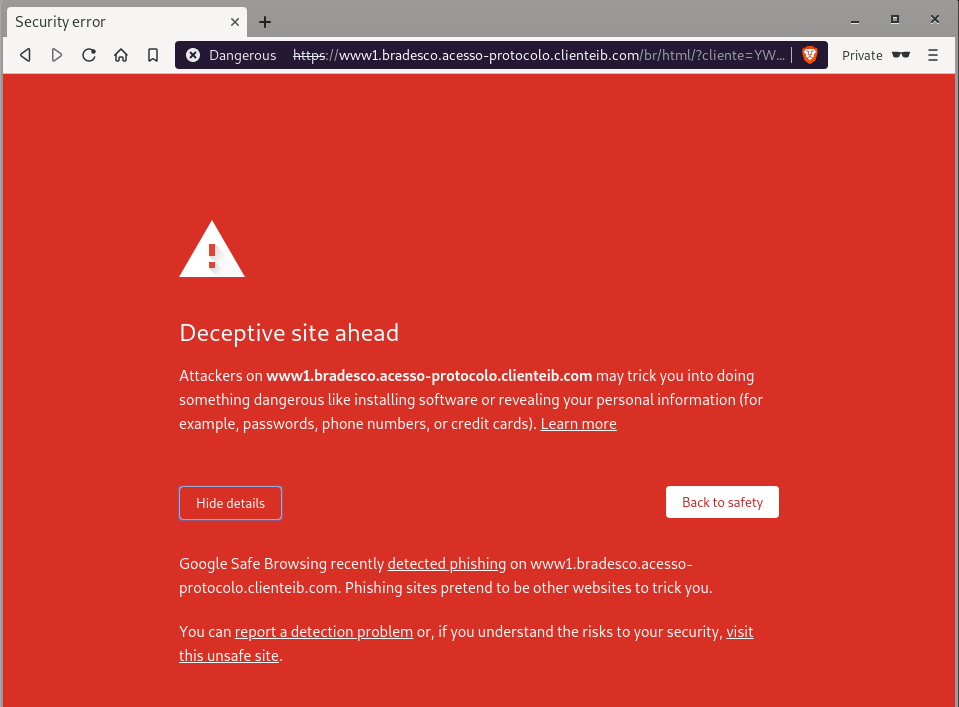
\includegraphics[width=1\textwidth]{images/browser_phishing_detected.png}
  \label{fig:browse-detection}
\end{figure}

\subsection{Anti-virus}



The majority of popular anti-virus technologies also provides some sort of defence mechanism. We will test several of them to compare it to our system in later stage of development. For the whole picture, there is current list of antivirus solutions:
\todo[inline]{Pridat screenshoty/videa do priloh, ako sa sprava antivirus ked sa navstivi dana webstranka}
\begin{itemize}
    \item ESET - \href{https://www.eset.com/us/anti-phishing/}{ESET}
    \item AVAST - \href{https://blog.avast.com/avast-improves-phishing-detection-avast}{Avast}
    \item Kaspersky
    \item Norton
    \item Bitdefender
\end{itemize}


\subsection{User education}

If the automatic detection mechanism fail, there is a space for a human factor. The user should be educated, how to look for a signs of phishing site. There are several methods how to educate a user such as briefings with security experts,
\todo{pridat citaciu s odporucanym zdrojom na edukaciu} pay the professional teams which tries to breach your company by phishing techniques \todo{pridat link/vysvetlit ako funguju skolenia} or by periodically sending the new/emails from security department on a current state of phishing attacks and how to prevent them.

\section{Phishing trends}

How does the phishing developed over the years? We can look at the data from the APWG \cite{apwg-2019-2}. They are periodically publishing their reports with trends for the previous quarter. They are including in the statistics the following:
\begin{itemize}
    \item The number of unique phishing websites. "The APWG tracks the Web sites across the globe. In their statistics, single phishing site may be advertised as thousands of customized URLs (all leading to the same attack destination)" \cite{apwg-2019-2}.
    \item The number of phishing (e-mail) campaigns. "The APWG tracks the number of unique phishing reports it receives from peers. An e-mail campaign is a unique e-mail sent out to multiple users, directing them to a specific phishing web site (multiple campaigns may point to the same web site). APWG counts unique phishing report e-mails as those found in a given month that have the same email subject line" \cite{apwg-2019-2}.
    \item The number of brand targeted by phishing campaigns. \cite{apwg-2019-2}
\end{itemize}

We've compiled the data from the reports published during a period since October 2012 till the June 2019 \cite{apwg-2012-4}--\cite{apwg-2019-2} and put it in the a graph (figure \ref{fig:apwg-trends} on page \pageref{fig:apwg-trends}) and table \ref{table:apwg-trends}.


\begin{figure}[]
%   \begin{center}
    \centering
    \rotatebox[origin=c]{270}{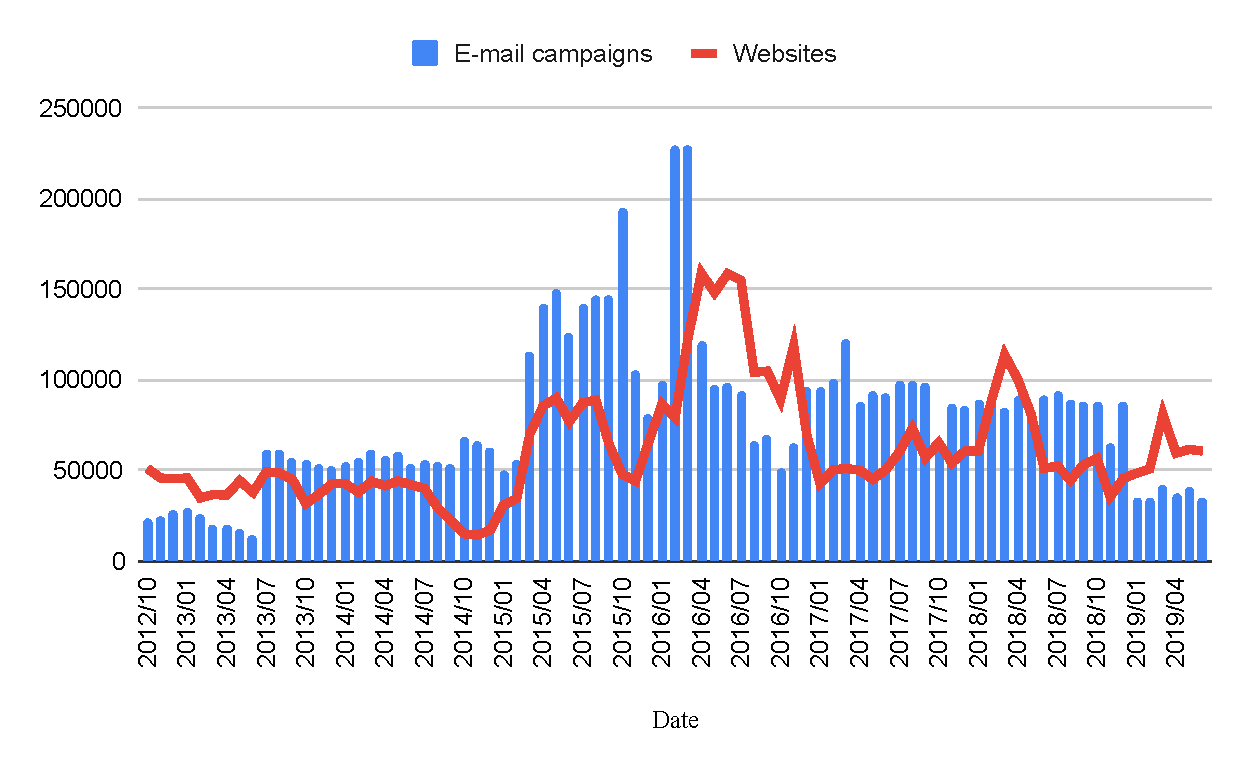
\includegraphics[width=17cm]{images/apwg-trend-chart.pdf}}
    \caption{Phishing campaigns and websites trends}
    \label{fig:apwg-trends}
%   \end{center}
\end{figure}

\begin{table}[h!]
    
    \begin{tabular}{r|ccc}
    \hline
    \multicolumn{1}{l|}{} & \multicolumn{1}{r}{E-mails campaigns} & Websites  & Brands \\ \hline
    Total                 & 6,400,431                             & 5,026,891 &        \\
    Monthly (median)      & 69,925                                & 51,232    & 358    \\
    Monthly (average)     & 79,018                                & 62,060    & 358    \\ \hline
    \end{tabular}\par
    \caption{E-mail campaigns, websites and brands statistics}
    \bigskip
    Data source: APWG 2012/10 -- 2019/06
    \label{table:apwg-trends}
\end{table}

Another study from year 2009 \cite{empirical-analysis-blacklists} claims, that average phishing campaign lasts about 2 hours (see in table \ref{table:phishing-sites-time}), but reaction time for taking down the site is much larger.

\begin{table}[h!]
\begin{tabular}{ccc}
\hline
\begin{tabular}[c]{@{}c@{}}Time elapsed\\ (hours)\end{tabular} & \begin{tabular}[c]{@{}c@{}}Websites taken \\ down (\%)\end{tabular} & \begin{tabular}[c]{@{}c@{}}Phishing campaigns\\  finished (\%)\end{tabular} \\ \hline
0                                                              & 2.10\%                                                              & 0\%                                                                         \\
2                                                              & 7.90\%                                                              & 63\%                                                                        \\
4                                                              & 17.80\%                                                             & 67\%                                                                        \\
5                                                              & 19.90\%                                                             & 70\%                                                                        \\
12                                                             & 33.00\%                                                             & 72\%                                                                        \\
24                                                             & 57.60\%                                                             & 75\%                                                                        \\
48                                                             & 72.30\%                                                             & 90\%                                                                        \\ \hline
\end{tabular}
\caption{Longevity of phishing sites in 2009 \cite{empirical-analysis-blacklists}}
\label{table:phishing-sites-time}
\end{table}

We can make an experiment, what are the real numbers for a phishing sites. There is an online service which can provide us the data. Phishtank \cite{phishtank} is an online collaborative tool to track and share phishing data. Anyone can submit a fraudulent URLs, users then manually verify whether a given website is malicious or not. We've described the method of obtaining data in later chapters. \todo[inline]{linknut tu kapitolu z implementacie s kodom, nech sa v uvode neriesa implementacne detaily}

First we will look at the total number of submitted phishing sites and brands (Phishtank is not evaluating e-mail campaigns). We can see in the table \ref{table:phishtank-stats} that average number of submitted phishing sites per month (11,904) is 5--6 times smaller (62,060) what is APWG reporting. This may be due to the fact, that APWG is a larger institution and have multiple data sources, whereas Phishtank is relying on users.

\begin{table}[h!]
\begin{tabular}{ccc}
\hline
                  & Websites & Brands \\ \hline
Total             & 119,043   &        \\
Monthly (median)  & 10,438    & 81   \\
Monthly (average) & 11,904    & 85   \\ \hline
\end{tabular} \par
\caption{Phishtank statistics} 
\bigskip
Data source: Phishtank 2018/11 -- 2019/08
\label{table:phishtank-stats}
\end{table}


In the figure \ref{fig:apwg-vs-phishtank} we can see the comparison over the same time period. We can see, that each data source has its own spike, but they are not in any relationship. Another thing that we can notice is, that APWG has bigger trending line than Phishtank.

\begin{figure}[h!]
  \begin{center}
    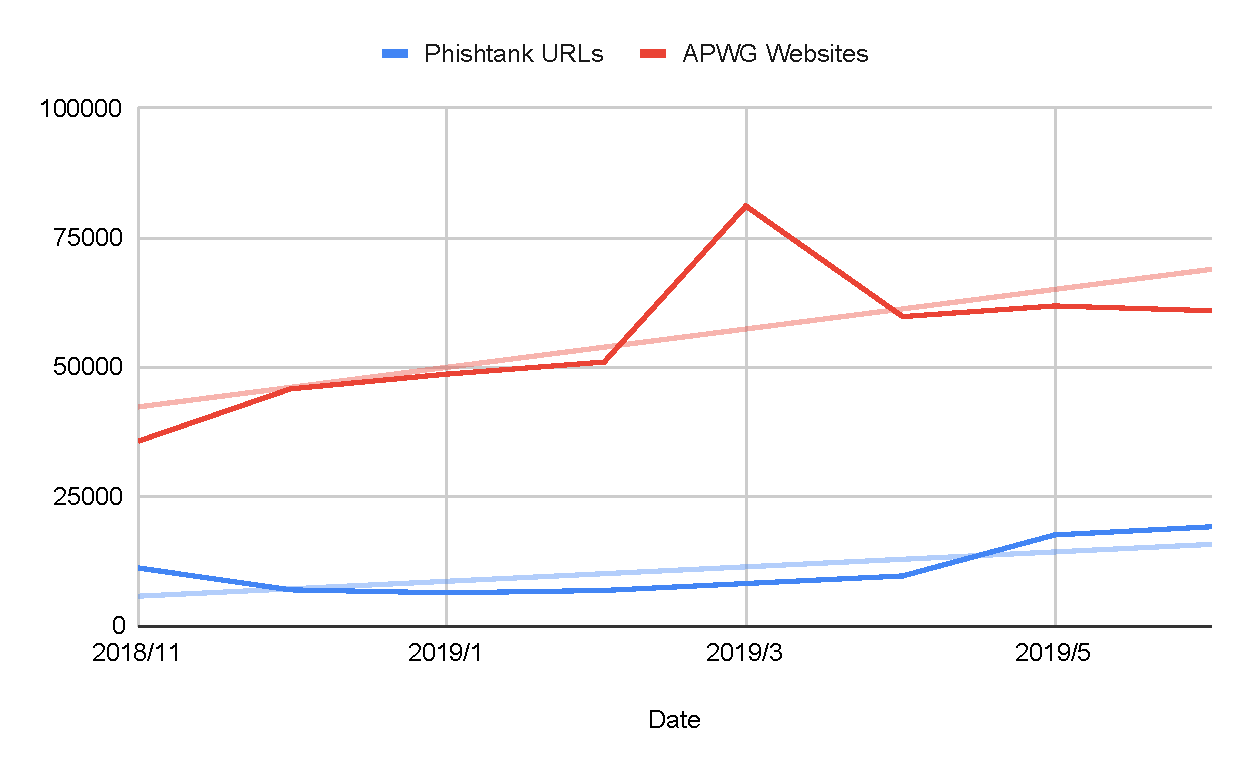
\includegraphics[width=12cm]{images/apwg-vs-phishtank.pdf}
    \caption{APWG vs Phishtank stats over 2018/11 - 2019/06}
    \label{fig:apwg-vs-phishtank}
  \end{center}
\end{figure}

Another statistics that we can derive from Phishtank's data is, how long does it actually take down registered URL on Phishtank. How we are obtaining the data is described in section \ref{??}. \todo[noinline]{link na implementaciu}


The obtained Phishtank's data are queried once per day, thus we don't know the hourly updates. We can check how many days (instead of hours) is usually the URL online after submission.

\begin{table}[h!]
\begin{tabular}{cc|cc}
\hline
    \begin{tabular}[c]{@{}c@{}}Time \\ elapsed\end{tabular} & \begin{tabular}[c]{@{}c@{}}Websites\\  taken down\end{tabular} & \begin{tabular}[c]{@{}c@{}}Time \\ elapsed\end{tabular} & \begin{tabular}[c]{@{}c@{}}Websites\\  taken down\end{tabular} \\ \hline
    0 days       & 2.9\%                & 2 Weeks        & 67.0\%               \\
    1 day        & 19.5\%               & A month        & 79.8\%               \\
    2 days       & 31.2\%               & A quarter year & 91.5\%               \\
    3 days       & 39.1\%               & A half year    & 95.0\%               \\
    A week       & 54.6\%               & A year         & 95.5\%               \\ \hline
    Still online & 4.5\%                &                &                      \\ \hline
\end{tabular}\par
\caption{Time to take URL down}
\bigskip
Data source: Phishtank 2018/11 -- 2019/08
\label{table:phishtank-urls-time}
\end{table}

This data are saying, that it takes more time to take down a website, than is claimed in the previous work.

\section{Technical terms and technologies}

For the better understanding of this work, we will explain and describe several terms and technologies, which are necessary for understanding of the next chapters.

\subsection*{HTTP}
\label{term:http}
\todo[inline]{Vysvetlit ako funguje HTTP, HTTPS. Ako vyzera request, response. Popisat metody (GET/POST/...).}
\subsection*{API}
\label{term:api}
\todo[inline]{Vysvetlit co je to API. Ako sa pouziva v dnesnom svete.}
\subsection*{URL}
\label{term:url}
\todo[inline]{Ukazat co je to URL/URI. Ake ma casti. Pekny obrazok vytvorit (alebo skopirovat a zdrojovat)}
\subsection*{IPv4, IPv6}
\label{term:ip}
\label{term:ipv4}
\label{term:ipv6}
\todo[inline]{Popisat IPv4, IPv6}
\subsection*{DNS}
\label{term:dns}
\todo[inline]{Popisat DNS. Napisat co je MX record, A, AAAA, TXT.}
\subsection*{HTML}
\label{term:html}
\todo[inline]{Popisat HTML a prvky. Vysvetlit ako vyzera webova stranka a ako funguju elementy.}

\chapter{Detection methods}
% TODO: this chapter will be about specific approaches and test - why I chose them and why are they beneficial for our app

\section{Manual methods}

\section{Automated methods}
\label{section:automated-methods}

Deciding whether the site is phishing or not is not trivial problem. There are many researches and papers with proposed systems that this work derives from. They are mentioning the following approaches.

\subsection{List based approach}
\label{section:list-based}

This approach is based on known lists, which are publicly known. We usually perform two operations with these lists - whitelisting and blacklisting. Whitelisted URLs are taken as non-malicious sites, whereas URLs listed on some blacklist are considered as malicious. Usually, there is no difference between malicious categories in general lists - we can't say that this URL contains malware but is not phishing or the other way. But there are some services that provides only phishing info.

The advantage of list based approach is, that we have a binary information about inspected URL - either it is a malicious site or not, no uncertainty. The disadvantage is that usually it takes much time to add it to these lists, they are not reactive as the we want them to be.

Lets see, what services exists for list based approach.

\subsubsection{Phishtank}

Phishtank \cite{phishtank} is an online collaborative tool to track and share phishing data. Anyone can submit fraudulent URLs, users then verify if a given website is a phishing site or not. Phishtank provides a public API  where a client can perform a lookup for one URL through the POST request \footnote{\href{https://www.phishtank.com/api_info.php}{https://www.phishtank.com/api\_info.php}}, or he can request a current snapshot of the database \footnote{https://www.phishtank.com/developer\_info.php}. 

\subsubsection{OpenPhish}

OpenPhish \cite{openphish} is automated platform for phishing intelligence. It analyses given URLs from various partners, and if an URL is a phishing one, its provides variety of metadata and information. Then the platform provides a list with live phishing URLs. 

\subsubsection{Google Safe Browsing}
\label{section:google-safe-browsing}

Google provides it's own lists through a Safe Browsing API \cite{google-safe-browsing}. The client application can query the API and get information if has any threat type (malware, social engineering or other).

Last two methods are slightly different than previous, because they are working only with hostnames/domains, instead of whole URLs.

\subsubsection{DNSBL}

Domain Name System-based Blackhole List \cite{wiki:dnsbl} is used for real time stopping of the spam. Spam campaings are usually going together \todo{najdi paper kde si toto cital} with phishing campaigns. Lookup in DNSBL is performed through DNS "A" records. If record is returned, than host is blacklisted. If domain is not listed (and thus its clear), NXDOMAIN is returned. \todo[inline]{vysvetlit/prelinkovat na A/NXDOMAIN recordy z predchadzajucej kapitoly}

\subsubsection{DNSWL}

DNS-based whitelist \cite{wiki:dnswl} has on a contrary other approach - locations of IP addresses or hosts, which are consistent and have low percentage of a spam. This option is mainly for future extensions, because black listing is not possible for many host in IPv6 universe.

List-based approach also has big disadvantage - it's not reactive enough. As stated in \cite{empirical-analysis-blacklists} an average phishing campaign lasts only about 2 hours. This is usually too short amount of time to send an URL to a service, categorize it manually, and deploy it in blacklist. Because of this, we need to look for another approaches. 

\subsection{URL analysis}
\label{section:url-analysis}

\todo[inline]{DOROBIT ANALYZU NA PHISHTANK DATABAZE A KERNUN DATABAZE}

Another possible approach is to perform an analysis of a URL. We can define several features that are interesting for us, and look at them in a detail, so they could give us a picture if a given URL is phishing and with what probability.

This method's advantage is, that we can perform in a real time and can decide whether an URL is malicious in lesser time than in list-based approach. On the other side, there will be surely some false positives or some URLs will misbehave. 

We have read and studied several academic works which are concerned with this topic. During following subsection we will introduce several URL features which looks promising, or other groups of authors successfully used them in their systems. We will also introduce new features, that we think may be useful, and we didn't see any other work to use them.

For each feature, we will provide a real world phishing example, and perform basic statistics on our three datasets:
\begin{itemize}
    \item Phishtank. We've compiled daily snapshots during 2018/10/25 -- 2019/09/28. The total number of records (without 22 malformed URLs that parser had a problem) is 163,891. The data sets contains submitted URLs from users which were confirmed as malicious. \todo[inline]{dodat informacie ako som vyrobil tento set v implementacnej casti a pridat link na repo}
    \item Kernun's customer traffic. We've got anonymised data from a customer's day traffic. Total number of records (without 2897 malformed URLs that parser had problem) is 6,565,290. 
    \item Alexa. We've downloaded a list of most accessed websites as per Alexa list. The data set contains only hostnames and has total of 939,039 records.  
\end{itemize}
To not pollute this section with implementation details, we will describe the exact steps how we got these statistics in sections \ref{xxx}.

\subsubsection{Usage of the IP address \cite{url-features-work} \cite{new-method-for-detection}
\cite{fresh-phish}} 

In normal case, every website need to be hosted somewhere (a host machine). This host machine is assigned with a public IP address, so everyone can access it globally. If a user had to remember for every site numeric combination of an IP address, it would be mess and we couldn't access more than a handful of sites. For this problem DNS (more info about DNS in section \ref{term:dns}) was developed. 

DNS providers charge some money to add a new DNS record. Phishers may try to lower their costs avoiding a DNS records and have only pure IP address. This behaviour is suspicious for an end-user, thus this is our first proposed feature.

\begin{feature}{IP address in classic notation}
\centerline{\url{http://138.197.136.185/bnc/National\%20Bank\%20Online.html}}
\end{feature}

The IP address also could be encoded into other formats, such as binary, octal, decimal and hexadecimal
\todo[inline]{pridaj citaciu \url{http://pc-help.org/obscure.htm\#dword}}.

\begin{feature}{Octal}
\centerline{\url{https://0254.0331.027.0356}}
\end{feature}

\begin{feature}{Decimal (google.com)}
\centerline{\url{https://2899908590}}
\end{feature}

http://1/

\begin{feature}{Hexadecimal (google.com)}
\centerline{\url{http://0x308f647/-credit-agricole-france/}}
\end{feature}
\subsubsection{Length of the URL \cite{fresh-phish} 59 65 71 72}

The length of an URL is common practice to hide the doubtful part from the user. There are several papers, that are saying that the length above some threshold is looking suspicious     (\cite{a-url-address-aware}, \cite{beyond-blacklists}, \cite{malicious-url-detection}, \cite{off-the-hook}). This metrics is one of the best classifier for machine learning algorithms according to \cite{off-the-hook}. 

Other studies are also stating, that we can use all parts from URL such as sub-domain, domain, path, query and path token count.

We have looked on our data, and results are following:

\begin{table}[h!]
\begin{tabular}{l|llll}
\multicolumn{1}{c|}{Hostname length (no TLD)} & Samples & Mean & Median & Max \\ \hline
Kernun                                        & 999,249  & 15   & 14     & 72  \\
Phishtank                                     & 163,890  & 16   & 14     & 245 \\
Alexa                                         & 939,039  & 15   & 14     & 73 
\end{tabular}
\caption{Hostnane length (without TLD)}
\label{table:hostname-length}
\end{table}

\begin{table}[h!]
\begin{tabular}{l|llll}
\multicolumn{1}{c|}{Path length} & Sample  & Mean & Median & Max   \\ \hline
Kernun                    & 999,554 & 24   & 13     & 384   \\
Phishtank                 & 158,325 & 31   & 24     & 2,063
\end{tabular}
\caption{Length of the path}
\label{table:path-length}
\end{table}

\begin{table}[h!]
\begin{tabular}{l|llll}
\multicolumn{1}{c|}{Query length} & Sample  & Mean & Median & Max   \\ \hline
Kernun                            & 869,181 & 164  & 123    & 382   \\
Phishtank                         & 34,888  & 90   & 59     & 4,094
\end{tabular}
\caption{Length of the query}
\label{table:query-length}
\end{table}

\begin{table}[]
\begin{tabular}{l|llll}
\multicolumn{1}{c|}{URL length} & Sample  & Mean & Median & Max   \\ \hline
Kernun                          & 999,555 & 195  & 145    & 400   \\
Phishtank                       & 163,890 & 78   & 56     & 4,173
\end{tabular}
\caption{Length of the whole URL}
\label{table:URL-length}
\end{table}

From this data, we can set the following features:
\begin{itemize}
    \item length of the hostname > 73
    \item length of the path > 384
    \item length of the query > 382
    \item length of the URL > 400
\end{itemize}

\begin{feature}{Length of the URL}
\url{https://n3plcpnl0109.prod.ams3.secureserver.net/\%7Efj7o34yqrpzi/irs?https://irs.gov}
\end{feature}





\subsubsection{Symbol @ \cite{url-features-work} \cite{cantina} \cite{fresh-phish}}

URL can have symbol @ (see \ref{term:url}), used as login information. Nowadays, this is not used because of security issues, but phishers can try to obfuscate the phishing URL, because majority of users are watching only on the start of an URL. Following example is resolved to \texttt{my-website.com}.

\begin{feature}{Symbol @}
\url{https://www.paypal.com@my-website.com}
\end{feature}

There was no single URL in our datasets, that contains \texttt{user\_info}. It can be caused by the fact, that it's easily detectable and today's detection mechanisms are blokcing it instantly, so the attackers don't bother to use this technique. 


%%%%%%%%%%%%%%%%%%%%%%%%%%%%%%%%%%%%%%%%%%%%%%%%

% \subsubsection{Prefix/suffix domain with a dash symbol (-) \cite{url-features-work} \cite{new-method-for-detection}
% \cite{fresh-phish}} 
% \label{url-feature:prefix}

% The phisher can try to mimic a legitimate site with altering a well known domain. Work \cite{url-features-work} is arguing, that dash is rarely used in legitimate URL. 

% % After my research of Top1000 websites and sample of phishing database, we can say that X\% of Top1000 websites uses dash in a domain and Y\% of Phishing database (from date ...) uses dash in a domain. Import a nice table.

% \begin{feature}{Prefix/suffix domain with a dash symbol (-)}
% \url{https://my-paypal.com} \\
% \url{https://paypal-me.com} \\
% \url{https://pay.pal-app-problemresolutionsummary.com}
% \end{feature}

%%%%%%%%%%%%%%%%%%%%%%%%%%%%%%%% 

\subsubsection{Nested sub-domains \cite{url-features-work} \cite{cantina} \cite{new-method-for-detection}
\cite{fresh-phish}}

The technique with nesting sub-domains is similar approach like with a long URL - trying to mask a host with a targeted brand. Academic works are mentioning, that 4 sub-domains are considered as a phishing. On the other hand, lot of websites now are using Amazon webservices for hosting their legitimate sites, and their URL can looks like \url{	https://ec2-18-223-122-56.us-east-2.compute.amazonaws.com/}. Also, the nested subdomains are usually used for internal systems with signing service. In our datasets, we found a following distribution:
\begin{table}[]
\begin{tabular}{l|lllll}
\multicolumn{1}{c|}{Nr. of subdomains} & 0      & 1      & 2      & 3    & 4+    \\ \hline
Kernun                                 & 202324 & 596923 & 187496 & 1771 & 10735 \\
Phishtank                              & 99909  & 48159  & 10446  & 3452 & 1911  \\
Alexa                                  & 939039 & 776981 & 160593 & 1441 & 24   
\end{tabular}
\caption{Distribution of subdomains}
\label{table:subdomain-distribution}
\end{table}
% Table: phishing/kernun/top2500 sites with <3/4/5/6+ subdomains. 

\begin{feature}{Nested sub-domains}
\url{http://history.meps.tp.edu.tw/sites/hstl/}
\end{feature}

\subsubsection{Usage of HTTPS \cite{methodical-overview} \cite{url-features-work}}

For a long time on the internet, ratio of HTTP vs HTTPS sites was in a favor for unencrypted sites. Then company Let's Encrypt starts providing a free HTTPS certificate, which can be obtained through an API and the overall look of the World Wide Web has changed. We can see in a figure \ref{fig:https-firefox} that in a year 2017 there was for the first time more HTTPS sites than HTTP, and since then the number rapidly grows. In our data-sets, the numbers are following:

\begin{table}[h!]
\begin{tabular}{l|ll}
HTTPS sites & Count  & Count (\%) \\ \hline
Kernun      & 738360 & 73.87\%    \\
Phishtank   & 66226  & 40.41\%   
\end{tabular}
\caption{Ratio of HTTPS sites in dataset}
\label{table:https-sites}
\end{table}

\begin{figure}[]
  \caption{Percentage of Web Pages Loaded by Firefox Using HTTPS}
  \centering
  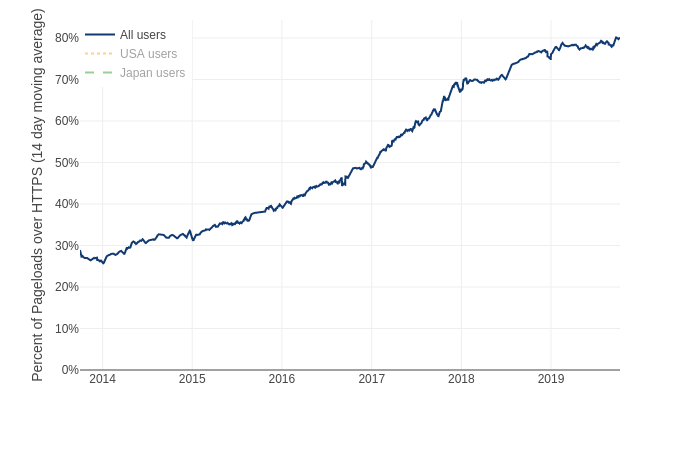
\includegraphics[width=0.8\textwidth]{images/https-firefox.png}
  \label{fig:https-firefox}
\end{figure}

We can still see that phishing sites are not using HTTPS as much are normal URLs. So we can say, that non-HTTPS sites are phishing.

\begin{feature}{Missing HTTPS}
\url{http://icloud.com.fmidevice.id-login.site/}
\end{feature}

\subsubsection{Extra \texttt{https} token \cite{fresh-phish}}

If \texttt{https} certificate is not acquired by a legitimate way, phishers may try to convince a user that site is secured by an extra token. There is an assumption, that lots of users don't pay an attention to hierarchy of an URL, and when they see a string \texttt{https}, they think that site is secure. In our datasets, findings where following:

\begin{table}[h!]
\begin{tabular}{l|ll}
\texttt{https} token & Count & Count (\%) \\ \hline
Kernun            & 0     & 0.00\%     \\
Phishtank         & 120   & 0.07\%     \\
Alexa             & 12    & 0.00\%    
\end{tabular}
\caption{Extra \texttt{https} token}
\label{table:extra-https}
\end{table}

From ths data, we can say that a hostname starting with a \texttt{https} is a phishing.

\begin{feature}{Extra \texttt{https} token}
\url{http://www.https-myetherwallet.net/}
\end{feature}

\subsubsection{Shortening service \cite{fresh-phish} \cite{phishstorm}}

Shortening service is a method of transforming a relatively long URL into a shorter one, which can user memorise, send over services which are limiting the length of a message or just make it smaller for other reasons. Technically is this done over HTTP redirect method 301 - shortening service server will redirect a client to the original URL.

Phishers may try to confuse a user with legitimate services (\url{bitly.com}, \url{goo.gl}), to initially obtain a feeling that link is normal one. When users are already on a website, they may not see that URL is now a long or suspicious. 

\begin{table}[h!]
\begin{tabular}{l|ll}
Extra HTTPS token & Count & Count (\%) \\ \hline
Kernun            & 0     & 0.00\%     \\
Phishtank         & 120   & 0.07\%     \\
Alexa             & 12    & 0.00\%    
\end{tabular}
\caption{Usage of shortening service}
\label{table:shortening-service}
\end{table}


\begin{feature}{Shortening service}
\url{https://tiny.cc/GnjUIz} \medbreak resolves to \\
\url{https://bankieren.rabobank.nl.scannerplus.be/nl/service/online-bankieren/nieuwe-rabo-scanner-aanvragen/bankpas_aanvragen.php}
\end{feature}


\subsubsection{Non-standard port \cite{fresh-phish}}

\begin{table}[]
\begin{tabular}{l|ll}
Non standard port & Count & Count (\%) \\ \hline
Kernun            & 561   & 0.06\%     \\
Phishtank         & 1324  & 0.81\%    
\end{tabular}
\caption{Usage of non standard port}
\label{table:non-std-port}
\end{table}

The standard ports are defined by organization IANA \footnote{https://www.iana.org/assignments/service-names-port-numbers/service-names-port-numbers.txt}, for \texttt{http} it is 80, for \texttt{https} 443. We can see in table \ref{table:non-std-port} that almost every site on internet is using standard port. The most used (1182 occurrences) port by phishing sites (except the standard) is port number \texttt{81}. 



\begin{feature}{Non-standard port}
\url{http://jppost-yo.com:81/dao.html}
\end{feature}

\subsubsection{Special characters}

Several works \cite{methodical-overview} \cite{novel-algorithm} \cite{malicious-url-detection} \cite{off-the-hook} are describing, that presence of special characters such as  '!', '@', '\#', '\$', '\%'
'\^', '\&', '*', '(', ')', '\_', '-', '+', '/', '\', or '=' can be used as another feature. We have analysed total count of special characters in the URL parts. The findings were following:

\todo[inline]{Pridat percentualne vyjadrenia danej statitisky, aby sa dalo pozriet ze ci su nejake vyznamne rozdiely medzi danymi datasetmi, aby sa dalo uvazovat nad tym ze sa to pouzije ako feature}

\begin{table}[h!]
\begin{tabular}{llllllll}
\multicolumn{1}{c}{Sp. chars in host} & Records & 0       & 1       & 2-3    & 4-5   & 6-10 & 11+ \\
Kernun                                & 999,555 & 748,859 & 169,201 & 78,021 & 2,059 & 289  & 0   \\
Phishtank                             & 163,890 & 125,965 & 28,382  & 7,892  & 284   & 290  & 15 
\end{tabular}
\end{table}

\begin{table}[h!]
\begin{tabular}{llllllll}
\multicolumn{1}{c}{Sp. chars in path} & Records & 0 & 1       & 2-3     & 4-5    & 6-10    & 11+    \\
Kernun                                & 999,554 & 0 & 330,296 & 438,447 & 32,413 & 130,478 & 29,005 \\
Phishtank                             & 158,325 & 0 & 35,653  & 56,120  & 12,897 & 29,379  & 5,929 
\end{tabular}
\end{table}

\begin{table}[h!]
\begin{tabular}{llllllll}
\multicolumn{1}{c}{Sp. chars in query} & Records & 0      & 1      & 2-3    & 4-5    & 6-10    & 11+     \\
Kernun                                 & 869,181 & 41,223 & 26,069 & 39,312 & 36,985 & 193,824 & 517,757 \\
Phishtank                              & 34,888  & 2,096  & 5,752  & 6,222  & 2,027  & 10,375  & 4,410  
\end{tabular}
\end{table}

\begin{table}[h!]
\begin{tabular}{llllllll}
\multicolumn{1}{c}{Sp. chars in fragment} & Records & 0   & 1   & 2-3 & 4-5 & 6-10 & 11+ \\
Kernun                                    & 1       & 0   & 1   & 0   & 0   & 0    & 0   \\
Phishtank                                 & 826     & 152 & 177 & 121 & 280 & 26   & 50 
\end{tabular}
\end{table}

We have also looked  at the specific characters, but only dash and underscore had some interesting results:

\begin{table}[h!]
\begin{tabular}{lll}
\multicolumn{1}{c}{Dash symbol in hostname} & Total  & Total (\%) \\
Kernun                                      & 250640 & 25.08\%    \\
Phishtank                                   & 37891  & 23.12\%    \\
Alexa                                       & 101821 & 10.84\%   
\end{tabular}
\end{table}

\begin{table}[h!]
\begin{tabular}{lll}
\multicolumn{1}{c}{Dash symbol in hostname} & Total & Total (\%) \\
Kernun                                      & 54    & 0.01\%     \\
Phishtank                                   & 35    & 0.02\%     \\
Alexa                                       & 251   & 0.03\%    
\end{tabular}
\end{table}



\subsubsection{Special keywords}

Another metrics can be number of special keywords that are present in fishing URLs. In work \cite{cantina+}, they are stating that words "secure”, “account”, “webscr”, “login”, “ebayisapi”, “signin”, “banking”, “confirm” are sensitive. We will check for these words in URL and also check in our set, which words are most common.

\begin{table}[h!]
\begin{tabular}{lllll}
\multicolumn{1}{c}{Nr. of keywords} & Total records & 1      & 2      & 3+    \\
Kernun                              & 999,555       & 14,303 & 2,165  & 2,042 \\
Phishtank                           & 163,890       & 23,470 & 13,368 & 5,400
\end{tabular}
\end{table}


\subsubsection{Domain similarity}

\subsubsection{Non standard TLD}

We have looked at Alexa 10,000 most visited URLs and extracted 15 most used TLD. We have also looked in our Phishing and Kernun dataset, and extracted most used TLD. The findings were following:

\begin{table}[]
\begin{tabular}{lll}
\multicolumn{1}{c}{Top 15 domains} & \# of 'cz' &                                                                                                                \\
Kernun                             & 2          & .com', '.cz', '.net', '.de', '.org', '.io', '.co', '.eu', '.pl', '.li', '.to', '.sk', '.ru', '.it', '.140'     \\
Phishtank                          & 22         & .com', '.net', '.org', '.ru', '.br', '.top', '.info', '.in', '.icu', '.uk', '.au', '.co', '.pl', '.xyz', '.ga' \\
Alexa                              & 37         & .com', '.net', '.ru', '.org', '.jp', '.cn', '.br', '.in', '.de', '.fr', '.it', '.edu', '.ir', '.gr', '.tv'    
\end{tabular}
\end{table}

\subsubsection{Extra www prefix}

\begin{table}[]
\begin{tabular}{lll}
\multicolumn{1}{c}{Extra www prefix} & Count & Count (\%) \\
Kernun                               & 15    & 0.00\%     \\
Phishtank                            & 107   & 0.07\%     \\
Alexa                                & 55    & 0.01\%    
\end{tabular}
\end{table}

\subsubsection{More than 4 consecutive number \cite{malicious-url-detection}}

\begin{table}[]
\begin{tabular}{lll}
\multicolumn{1}{c}{More than 4 numbers} & Count & Count (\%) \\
Kernun                                  & 6042  & 0.60\%     \\
Phishtank                               & 837   & 0.51\%     \\
Alexa                                   & 2005  & 0.21\%    
\end{tabular}
\end{table}



All this features can be evaluated immediately - there is no need to query other services or analyse it. But there is another set of features which requires an analysis of a webpage.



%%%%%%%%%%%%%%%%%%%%%%%%%%%%%%%
\subsection{Analysis of a HTML}
\label{section:html-analysis}

\subsubsection{Input field \cite{url-features-work} \cite{anomaly-based-detection} \cite{cantina} }
The main reason for existence of phishing sites is, that an attacker wants to obtain credentials from a victim. If there is no present \texttt{<input>} field, there is less chance that attacker will get victim's credentials.

\begin{feature}{Input field}
\texttt{<input type="password">}
\end{feature}

\subsubsection{\texttt{src} attribute \cite{url-features-work} 
\cite{cantina} }

Several HTML tags may have \texttt{src} attribute. This attribute is used e.g. for sourcing the images or other assets. If the phishing site is simple copy of some other, than we can check whether domain in URL and \texttt{src} attributes matches.

\begin{feature}{\texttt{src} attribute}
\texttt{<img src="http://url.com">}
\end{feature}

\subsubsection{Anchor element \cite{methodical-overview} \cite{url-features-work} }

\footnote{https://developer.mozilla.org/en-US/docs/Web/HTML/Element/a}
\footnote{<script> <meta> <link>}
Anchor element is \texttt{<a>} element with its \texttt{href} attribute creates a hyperlink to local files, sources, e-mails or other URLs. In \cite{fresh-phish} they are using the metrics, that if 50\% links are pointing to other websites, the site is considered as phishing.

\begin{feature}{Anchor element}
\texttt{<a href="another-domain"></a>}
\end{feature}

\subsubsection{Form handler}

This feature is examining submit form handler \footnote{\url{https://www.w3schools.com/php/php_forms.asp}}. The legitimate site is usually having some meaningful action with a form data. Phishing sites may use \texttt{\#skip}, \texttt{blank}, \texttt{about:blank} or others.
Whole list of operations is in implementation: about:blank, none, skip, mailto
\begin{feature}{Form handler}
\texttt{<form action="about:blank" method="get"></form>}
\end{feature}

\subsubsection{HTTP redirect}
\todo[inline]{popisat ako funguje curl -I https://bit.ly/30KgsZ4}

This feature is a superset of feature with URL shorteners. HTTP redirect can be used by an attacker to hide the malicious URL behind another URL. If an URL is redirected more than some threshold, than it is considered as phishing URL.

\begin{feature}{HTTP redirect}
\url{http://ameland-diving.nl/market.php?8o42} \\
redirects to \\ 
\url{https://weightloss-life.com/amxl/intl/kt-s-desk?bhu=CWpZoK57zqskgGPsnCYcgGJy1fuuyHNKjUy9o}
\end{feature}

\subsubsection{Invisible \texttt{iframe}}

This feature is looking for iframes with invisible borders - an attacker may try to insert an iframe over a valid site with input fields sending the information to the fishing site.

\footnote{https://packetstormsecurity.com/files/121389/Iframe-URI-Phishing.html}

\begin{feature}
\texttt{<iframe src="https://www.w3schools.com"></iframe>}
\end{feature}


\subsubsection{onMouseOver \cite{fresh-phish} \cite{url-features-work} }

Attacker can change an URL address bar to something else with the use of \texttt{onMouseOver}.

\begin{feature}{onMouseOver}
\texttt{<a onMouseOver="window.status=https://bad-url.com" href="..."/>}
\end{feature}

\subsubsection{Disabled right click on a page \cite{methodical-overview} \cite{url-features-work} \cite{fresh-phish} }
Disabling right-click on page is considered as bad practice. Normal sites don't have a reason for a blocking it. So therefore, there is consideration that blocking a right click is only on a malicious site.

\begin{feature}{Disabled right-click}
\texttt{<body oncontextmenu="return false;">}
\end{feature}

\subsubsection{PopUp Window \cite{methodical-overview} \cite{url-features-work} \cite{fresh-phish} \cite{whitenet} }
\footnote{\url{https://www.w3schools.com/js/js_popup.asp}}
It's uncommon to ask for a user credentials through a pop up window. Because of that, we are checking pop up windows with some submit information.

\begin{feature}{PopUp window}
TODO: add a picture with a popup
\texttt{window.prompt("sometext","defaultText");}
\end{feature}


\subsubsection{Favicon}

The favicon of a website increases its credibility. We can look if a website has a favicon and if its point to current domain, or its trying to mimic other popular site.

\begin{feature}{Favicon}
\texttt{<link rel="shortcut icon" href="https://example.com/myicon.ico">}
\end{feature}

\subsubsection{Modern frontend framework}

We can try to examine if phishers adapted to the newly use of Angular, Vue, React. Myabe all of the phishing sites are using old technoglogies.




%%%%%%%%%%%%%%%%%%%%%%%%%%%%%%%
\subsection{Visual analysis}
\label{section:visual-analysis}
\cite{favicon}
- favicon visuality



%%%%%%%%%%%%%%%%%%%%%%%%%%%%%%%%%
\subsection{Behavioral analysis / external statistics}
\label{section:behavioral-analysis}

In the last category we can examine several type of properties of a site, which requires additional tools (WHOIS, dig, ...).

\subsubsection{Google index}

A page is indexed by Google if it has been visited by the Google crawler ("Googlebot"), analyzed for content and meaning, and stored in the Google index. Indexed pages can be shown in Google Search results. 
\footnote{https://www.google.com/search/howsearchworks/crawling-indexing/}
\footnote{https://developers.google.com/search/apis/indexing-api/v3/quickstart}
\footnote{https://support.google.com/webmasters/answer/7643011?hl=en}

\begin{feature}{Google index}

\end{feature}

\subsubsection{PageRank}

PageRank \footnote{https://patents.google.com/patent/US7058628B1/en} is an algorithm created by Google in its first days. The algorithm is measuring the importance of website pages. We can use PageRank to detect as a feature and say, if the site has some low page rank, usually because phishing sites are only for a short time online, then it's a phishing one.

\begin{feature}{PageRank}

\end{feature}
\url{https://www.prchecker.info/check_page_rank.php}

\subsubsection{Alexa}

\footnote{https://www.alexa.com/siteinfo}

Amazon's product Alexa is for analysis of a site. It is providing some metrics such as searched keywords paired with its traffic, similar sites, global rank in internet engagement and other. We can leverage some of these metrics, especially page rank, to say if the site is phishing.

\begin{feature}{Alexa siteinfo}

\end{feature}

\subsubsection{DuckDuckGo index}

\subsubsection{DNS record}

We can also gain some information from DNS \ref{term:dns} records. If there is no existing DNS record for a website, we can consider it as a risk. Also we can check the hostname or the identity field if its matching declared site.

\subsubsection{DNSSEC}

\subsubsection{DNS created} 2+ year
\subsubsection{DNS updated} recently updated
\subsubsection{TLS fingerprint}
\subsubsection{HTTPS certificate} claimed identity, authorities
\subsubsection{Content security policies} Working against XSS.


\chapter{System design}

Now that we have some knowledge about phishing detection methods and how prevention works, we can design our system. 

We reckon the main task of our system is deciding whether an URL is phishing, returning a phish score. We can split this problem into several smaller parts (see figure \ref{fig:activity-diagram}):
\begin{enumerate}
    \item Look into our database or a cache, whether we have already phishing score for a given URL
    \item Check the URL with a list based methods (subsection \ref{section:list-based}). This has a higher priority, because if an URL is already listed on some service as a phishing one, we can assume that someone take their time to put it there and classify as malicious site.
    \item Check the URL with another detection methods:
    \begin{itemize}
        \item URL analysis (subsection \ref{section:url-analysis}). This detection will be performed on the URL link. It will be done in a real-time (doesn't have a side-effects such as relying on a network latency) on a set of URL features, that we will choose from the list that we provided in section \ref{section:url-analysis}. 
        \item HTML analysis (subsection \ref{section:html-analysis}). This detection methods will be performed on the downloaded HTML page from the URL. We also need to think about network latency, or maybe the site will be down and set some time-out for this methods.
        \item Behavioral analysis (subsection \ref{section:behavioral-analysis}). This detection methods consists of use of another tools (whois, dig, etc). We need to think about network latency and set up time-out.
    \end{itemize}
    \item Combine results from detection methods and create a phishing score for a given URL.
    \item Set expiry date for given score (to respond for cases, that site will change over time, and it can change it's content), store it with additional metadata into database and return it
    \item Send a request to blacklisting services if the phishing score is above some threshold
\end{enumerate}

\begin{figure}[]
  \begin{center}
    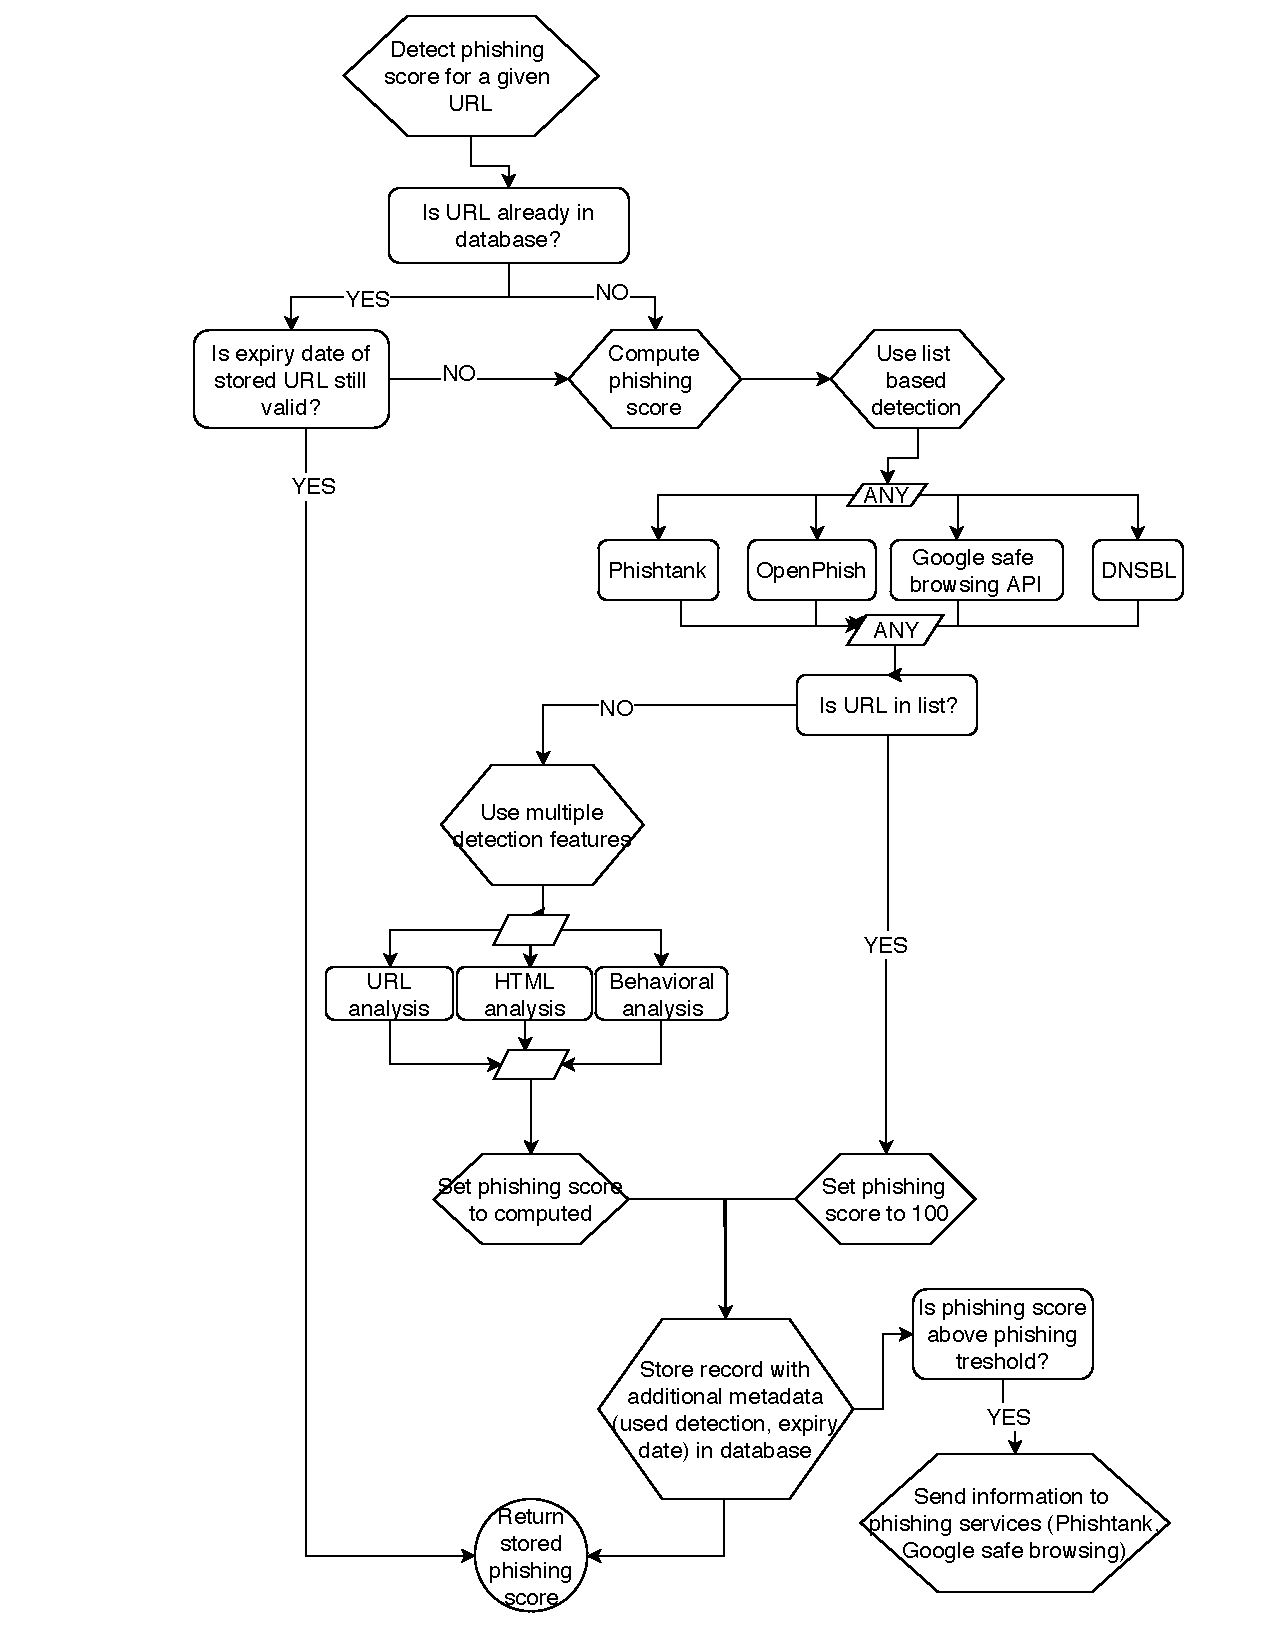
\includegraphics[width=12cm]{images/activity-diagram.pdf}
    \caption{Activity diagram}
    \label{fig:activity-diagram}
  \end{center}
\end{figure}

We have introduced in the previous chapter altogether \thefeature~features. How do we know, which of them are relevant? How do we know, that they will correctly detect a phishing site and correctly detect a normal one? Instead of tuning features manually (e.g. finding the correct thresholds or trying to find which feature is useless for) we can use methods of machine learning algorithms. % There are numerous works ([24]-[55], [XYZ]\todo{zacitovat papers s ML}) that are using this techniques.

\section{Machine learning basics}

A machine learning algorithm is an algorithm that is able to learn from data \cite{deep-learning}. We can split them into two basic categories: \textit{supervised} and \textit{unsupervised}.

Unsupervised machine learning algorithms takes data as input, without any previously classification or labeling, and try to find some structure or patterns in the data. Typical usage of these algorithms are with neural networks or deep learning.

Supervised machine learning algorithms takes not only the data, but also classification of the data. They are meant to used on a different set of problems, such as categorization, anomaly detection. The algorithms are fed with the data and classifiers.

So how does the process work? ML algorithms needs the data, which is in this field usually called \textit{training data}. Training data consists of multiple training examples. One training example, mathematical model, usually looks like a array or (feature) vector. Lots of these vectors, training examples, compose a matrix -- training data. 

We are then trying mapping input data to a desired output through an interative optimization of a function. Algorithm learn a a function that can predict output with not-previously seen input. Accuracy of the model is in direct correlation with a data -- more robust and quality data results in a better model.



\subsection{Data sets}

The works are working with a different number for a size of dataset: \cite{fresh-phish} has 35,000. Another work has around 12,000.

Our training data will consist from 3 data sources: confirmed phishing URLs, top visited sites on internet and normal traffic in a Czech company as we are trying to target the Czech market. 

\subsubsection{Top visited sites}

For the top visited sites, we have chosen the site Alexa \cite{alexa}. They are providing every 90 days a snapshot\footnote{\url{http://s3.amazonaws.com/alexa-static/top-1m.csv.zip}} of top 1 million visited sites based on their metrics. For the training data we will use top 10,000 sites.

\subsubsection{Phishing sites}

For the phishing URLs we have chosen site Phishtank. Phishtank \cite{phishtank} \label{section:phishtank} is an online collaborative tool to track and share phishing data. Anyone can submit fraudulent URLs, users then verify if a given website is a phishing site or not. Phishtank provides a public API  where a client can perform a lookup for one URL through the POST request \footnote{\url{https://www.phishtank.com/api\_info.php}}, or he can request a current snapshot of the live (websites not taken down) database \footnote{\url{https://www.phishtank.com/developer\_info.php}}. 

For data gathering, we have created a small JavaScript program \todo{Nalinkuj miesto v appendixe/zozname priloh kde bude offline kod} \footnote{\url{https://github.com/astaruch/phishurl-fetcher}} that will query Phishtank for their current database and updates our own database. We have gathered data from 25th of October 2018 until 26th of September 2019. One snapshot of live phishing URLs is typically around 10-12,000 URLs. Our final size of unique phishing URLs during that time period is 163,913 URLs.

Phishtank is providing records with several metadata (full documentation is in \ref{appendix:phishtank_record}) but only for live sites. We are recreating also a new parameter \texttt{end\_time} \todo{linknut kod s algoritmom kde to robim}, so we can do some statistics with these data.

\subsubsection{Normal traffic}

As the addition to Alexa sites for non-phishing URLs, we have gathered a daily log on 1st of November, 2018 from Kernun UTM+ Firewall containing 6,568,187 URLs. These records are not the URLs that user was clicking on, but all performed request which came through a proxy (together with a count how many times were the URL queried). The first ten records looks following:


\begin{table}[h!]
\begin{tabular}{ll}
Count   & URL                                                                                                    \\ \hline
6,613,465 & http://download.seznam.cz/software/conf/master.cfg                                                     \\
1,508,294 & https://log.pinterest.com/?event=auth\_fail\&type=extension\&xuid=H2QLtjPope\_A\&xv=cr3.0.991          \\
1,312,514 & http://okiprint-emea.com/pfe\_ws/Main.asmx                                                             \\
858,237  & http://searchclient.live.net/BingBar/signed/SeaPort.cab                                                \\
614,779  & http://www.okiprint-emea.com/pfe\_ws/Main.asmx                                                         \\
408,486  & http://g.ceipmsn.com/8SE/413?MI=5DE8D416C0EE4E0FAB4241C70A679E80-0\&LV=7.0.850.0\&OS=6.1.7601\&AG=2478 \\
365,840  & http://go.microsoft.com/fwlink/?LinkID=252669\&clcid=0x409                                             \\
300,073  & https://log.pinterest.com/?event=auth\_fail\&type=extension\&xuid=zPvGWndgsDik\&xv=cr3.0.991           \\
295,353  & http://weather.service.msn.com/data.aspx?wealocations=\&culture=cs-CZ\&weadegreetype=F\&src=outlook    \\
286,027  & https://ls.hit.gemius.pl/lsget.html                                                                   
\end{tabular}
\end{table}

\subsubsection{Training data}

For the purpose of model training, we will need training data and testing data. We will use ratio 80:20 (80\% of the training data, 20\% test data). As we are limited by number of phishing sites, we will select randomly 144,000 out of 163,913 records for the phishing dataset. For the normal URLs, we will select 10,000 most visited sites from Alexa and then 134,000 randomly selected URLs from the Kernun firewall.

Then we will divide 144,000 into 2 sets: 120,000 for the training and 24,000 for testing. Data sets are attached in the ...\todo{pridat link ked to bude v repe}.

\subsubsection{Fresh-phish}
\todo[inline]{Na validaciu systemu mozme pouzit existujuci framework a porovnat to potom s nasimi vysledkami \cite{fresh-phish}}

\subsection{Feature implementation}
We have now list of URLs and we need to transform it to training data. We will take features from section \ref{section:url-analysis} - \ref{section:behavioral-analysis}. If feature is marked as a phishing, we will give it value 1. If the feature is used for legitimate site, we will give it value 0. For non discrete values, we create a function, that will map values to interval [0, 1].

For each feature, we will provide algorithm in this section and link the implementation code in to appendix. Also, for each feature, we will implement a few tests so we will be sure, that everything work as expected.

Variable $v_n$ denotes value for feature $n$.

\subsubsection{IP address}

  \[
    v_1 =\left\{
                \begin{array}{lr}
                  1 & \mbox{if hostname is IP address};\\
                  0 & \mbox{otherwise}.
                  
                \end{array}
              \right.
  \]

\subsection{Feature selection}
\subsubsection{LASSO}
\subsubsection{Genetic algorithm}
\subsection{Model training and classification}
\subsubsection{SVM + rbf kernel}
\subsubsection{Random decision forest}
\subsection{Model evaluation and results}

\section{Architectural design}
\subsection{Functional requirements}
\subsection{Non-functional requirements}


\chapter{Application}


% TODO: whois, dns resolving, IP, /robots.txt...

% \section{?Frontend?}
% TODO: MAYBE IF THERE WILL BE TIME. Do a simple frontend for network administrator, so he can manually change behaviour of the app; e.g. add more values to some tests - enter google api key, refresh phishtank db, add new DNSBL and so on.

\chapter{Testing}

\section{Deployment}
% TODO: ideally create a Docker image for simple deployment on something like phishing-proxy.staruch.sk

\section{Integration into proxy}
% TODO: research possibility how to insert app into Kernun UTM/FW 

\section{Testing on real traffic}
% TODO: ideally, at least 2 weeks of testing - around march/april

\section{Results}
% TODO: prepare some graphs if this work is helpful or not, if speed of network is slower or unaffected, if customers are generally more happy, if newtork administrators can see some differences

\chapter{Summary}
% TODO: discuss what I did and if this thesis fulfills its goal



\shorthandon{-}


\printbibliography[heading=bibintoc] %% Print the bibliography.

\appendix
\listoftodos[Notes]

\chapter{Documentation}

\section{Phishtank record}
\label{appendix:phishtank_record}

% \begin{table}[]
\begin{tabularx}{\linewidth}{ r X }
\toprule
\textbf{phish\_id} & The ID number by which Phishtank refers to a phish submission. All data in PhishTank is tied to this ID. This will always be a positive integer. \\
\textbf{phish\_detail\_url} & PhishTank detail url for the phish, where you can view data about the phish, including a screenshot and the community votes. \\ \textbf{url} & The phish URL. This is always a string, and in the XML feeds may be a CDATA block. \\
\textbf{submission\_time} & The date and time at which this phish was reported to Phishtank. This is an ISO 8601 formatted date. \\
\textbf{verified} & Whether or not this phish has been verified by our community. In these data files, this will always be the string 'yes' since we only supply verified phishes in these files. \\
\textbf{verification\_time} & The date and time at which the phish was verified as valid by our community. This is an ISO 8601 formatted date. \\
\textbf{online} & Whether or not the phish is online and operational. In these data files, this will always be the string 'yes' since we only supply online phishes in these files. \\
\textbf{target} & The name of the company or brand the phish is impersonating, if it's known. \\ \bottomrule
\end{tabularx}
% \end{table}

\section{Phishurl fetcher}
\label{appendix:phishurl_fetcher}

\dirtree{%
.1 phishurl-fetcher. 
.2 README.md.
.2 docker-compose.yaml.
.2 ormconfig.json.
.2 package-lock.json.
.2  package.json.
.2  src.
.3     config.
.4     index.js.
.3     database.
.4     entity.
.5     LastUpdated.js.
.5     Phishtank.js.
.4     index.js.
.4     migration
.5     1555874663933-CreatePhishtank.js.
.5     1555897004589-CreateLastUpdated.js.
.4     model.
.5     LastUpdated.js.
.5     Phishtank.js.
.2     index.js.
.2     operations.
.3     last-updated.js.
.3     phishtank.js.
.2     utils.
.3     logger.js.
.3     utils.js.
}


\end{document}


% \begin{lstlisting}[language=Bash]
% $ git clone git@github.com:astaruch/master-thesis-phishtank-data.git
% $ cd master-thesis-phishtank-data
% $ bash unzip-data.sh

% $ git clone git@github.com:astaruch/phishurl-fetcher.git
% $ cd phishurl-fetcher
% $ docker-compose up -d
% $ npm run migrate
% $ node src/index.js -i -p ../master-thesis-phishtank-data/csv | pino-pretty

% $ docker pull dpage/pgadmin4
% $ docker run -e PGADMIN_DEFAULT_EMAIL=staruch.andrej@gmail.com -e PGADMIN_DEFAULT_PASSWORD=password -p 8080:80 -d dpage/pgadmin4 --name pgadmin

% $ docker network ls
% $ docker network inspect bridge
% $ # create bridge between database and a pgadmin
% $ docker network connect bridge phishing-detection-db
% $ docker network connect bridge pgadmin # this should be already in bridge network
% $ docker network inspect bridge # we should be able to do ping in both containers

% $ docker ps
% $ docker exec -it <pgadmin_HASH> sh
% $ docker exec -it <phishing-detection-db_HASH>
% \end{lstlisting}

% \begin{lstlisting}
% Old submissions
% SELECT COUNT(*) FROM phishtank WHERE submission_time BETWEEN '2012-10-01'::DATE AND '2019-06-30'::DATE 
% > 116630
% > AVG = 116630 / 81 = 1440

% I am fetching data since 2018/10/25, so we can use statistics for whole months
% 2018-11 -> 2019-08

% > SELECT COUNT(*) FROM phishtank WHERE submission_time BETWEEN '2018-11-01'::DATE AND '2019-09-01'::DATE > 119043
% > AVG = 119043 / 10 = 11904

% > BRANDS PER MONTH
% > SELECT EXTRACT(MONTH FROM submission_time) AS mon,
%       EXTRACT(YEAR FROM submission_time) AS yyyy,
%       COUNT(DISTINCT(target)) AS "monthly"
% FROM phishtank
% GROUP BY 1,2
% ORDER BY yyyy

% > HITS PER MONTH
% > SELECT EXTRACT(MONTH FROM submission_time) AS mon,
%       EXTRACT(YEAR FROM submission_time) AS yyyy,
%       COUNT(*) AS "monthly"
% FROM phishtank
% GROUP BY 1,2
% ORDER BY yyyy

% \end{lstlisting}

